\chapter{Appendix}

\section[Lagrangian of the Full Lossless Reciprocal Impedance Function]{Lagrangian of the Full Lossless Reciprocal Impedance\\ Function}\label{appendix:infty_freq_residue}
Now we consider the rational impedance function (\ref{eq:impedance}) but including the infinite frequency residue:
\begin{equation}
    \vb{Z}(s) = \frac{\vb{R}_0}{s} + \sum_{k=1}^M \frac{s \vb{R}_k}{s^2 + \omega_{R_k}^2} + s\vb{R}_\infty
\end{equation}
This corresponds to the full Cauer circuit shown in Fig.\ \ref{fig:cauer_circuit}. We can construct the Lagrangian in a similar way to what was done for the circuit without the purely inductive stage. Including the purely inductive stage, the Lagrangian now reads:
\begin{equation}
    \mathcal{L} = \frac{1}{2}\dot{\vb{\Phi}}_C^T \vb{C}_0 \dot{\vb{\Phi}}_C^{\phantom{^T}} + \frac{1}{2}\dot{\vb{\Phi}}_R^T \vb{C}_R \dot{\vb{\Phi}}_R^{\phantom{^T}} - \frac{1}{2}\vb{\Phi}_R^T \vb{M}_R \vb{\Phi}_R^{\phantom{^T}} - \frac{1}{2}\vb{\Phi}_L^T \vb{M}_L \vb{\Phi}_L^{\phantom{^T}} - \sum_{i=1}^N U_i(\Phi_{P_i})
\end{equation}
where everything is defined the same as before but now we also have $\vb{M}_L=\diag(L_1^{-1},\dots,L_N^{-1})$. Now we have the following constraints for the branch and node flux vectors:
\begin{align}
    \vb{\Phi}_C &= \vb{U}^T \vb{\Phi}_{PC} \\
    \vb{\Phi}_{PC} &= \vb{\Phi}_P - \vb{R}^T \vb{\Phi}_R - \vb{T}^T \vb{\Phi}_L
\end{align}
Using the above, we can obtain a Lagrangian that is only dependent on $\vb{\Phi}_P$, $\vb{\Phi}_R$, and $\vb{\Phi}_L$. The substitution $\vb{\Phi}_C \rightarrow \vb{U}^T (\vb{\Phi}_P - \vb{R}^T\vb{\Phi}_R  - \vb{T}^T \vb{\Phi}_L)$ allows us to write the following Lagrangian:
\begin{equation}
    \mathcal{L} =  \frac{1}{2}\dot{\vb{\Phi}}^T \vb{C} \dot{\vb{\Phi}} - \frac{1}{2}\vb{\Phi}^T \vb{M} \vb{\Phi}- \sum_{i=1}^N U_i(\Phi_{P_i})
\end{equation}
where we now have
\begin{align}
    \vb{\Phi} &= (\Phi_{P_1},\dots,\Phi_{P_N},\Phi_{R_1},\dots,\Phi_{R_M},\Phi_{L_1},\dots,\Phi_{L_N})^T\\
    \vb{C} &= \mqty(
        \vb{R}_0^{-1} & -\vb{R}_0^{-1}\vb{R}^T & -\vb{R}_0^{-1}\vb{T}^T \\
        -\vb{R}\vb{R}_0^{-1} & \vb{C}_R + \vb{R}\vb{R}_0^{-1}\vb{R}^T & \vb{R}\vb{R}_0^{-1}\vb{T}^T \\
        -\vb{T}\vb{R}_0^{-1} & \vb{T}\vb{R}_0^{-1}\vb{R}^T & \vb{T}\vb{R}_0^{-1}\vb{T}^T
    ) \\
    \vb{M} &= \mqty(
        \vb{0}_{N \times N} & \vb{0}_{N \times M} & \vb{0}_{N \times N} \\
        \vb{0}_{M \times N} & \vb{M}_R & \vb{0}_{M \times N} \\
        \vb{0}_{N \times N} & \vb{0}_{N \times M} & \vb{M}_L
    )
\end{align}
Here we can see that this impedance function does have a CL representation similar to the case of the impedance without the infinite frequency pole and residue. However, we cannot construct a circuit Hamiltonian since $\vb{C}$ is singular. To show this, we can partition $\vb{C}$ into 4 blocks:
\begin{equation}
    \vb{C} = \mqty( \bar{\vb{A}} & \bar{\vb{B}} \\ \bar{\vb{C}} & \bar{\vb{D}})
\end{equation}
where
\begin{align}
    \bar{\vb{A}} &= \vb{R}_0^{-1} \\
    \bar{\vb{B}} &= \mqty( -\vb{R}_0^{-1}\vb{R}^T & -\vb{R}_0^{-1}\vb{T}^T ) \\ 
    \bar{\vb{C}} &= \mqty( -\vb{R}\vb{R}_0^{-1} \\ -\vb{T}\vb{R}_0^{-1} ) \\
    \bar{\vb{D}} &= \mqty(  \vb{C}_R + \vb{R}\vb{R}_0^{-1}\vb{R}^T & \vb{R}\vb{R}_0^{-1}\vb{T}^T \\
    \vb{T}\vb{R}_0^{-1}\vb{R}^T & \vb{T}\vb{R}_0^{-1}\vb{T}^T )
\end{align}
The matrix $\vb{C}$ is invertible if $\bar{\vb{D}} - \bar{\vb{C}}\bar{\vb{A}}^{-1}\bar{\vb{B}}$ is invertible \cite[Proposition 2.8.7]{matrix_mathematics}. Computing this matrix, we find
\begin{equation}
    \bar{\vb{D}} - \bar{\vb{C}}\bar{\vb{A}}^{-1}\bar{\vb{B}} = \mqty( \vb{C}_R & \vb{0}_{M \times N} \\  \vb{0}_{N \times M} & \vb{0}_{N \times N})
\end{equation} 
This matrix is clearly singular and thus $\vb{C}$ is also singular. 

\newpage
\section{Degenerate Resonant Modes}\label{appendix:degen_res_mode}
To see how degenerate resonant modes arise and how the degeneracy can be broken, we consider the 3-port network shown in Fig.\ \ref{fig:tetrahedral_circuit}. This network is based off of the tetrahedral qubit structure presented in \cite{feigelman_superconducting_2004}. 

\begin{figure}[h!]
    \centering
    \begin{circuitikz}[line width=1pt]
        \ctikzset{bipoles/thickness=1, bipoles/length=1cm, , monopoles/ground/thickness=0.85}
        \ctikzset { label/align = straight }
        
        % Triangle structure
        \draw (-3,0) -- (-2,0) to[C,l=$C_c$] (-1,0) -- (0,0) -- (1,0) to[C,l=$C_c$] (2,0) -- (3,0) to[C,l=$C_c$] (1.5,-2.25) to[C,l=$C_c$] (0,-4.5) to[C,l=$C_c$] (-1.5, -2.25) to[C,l=$C_c$] (-3,0);

        % Resonator 1
        \draw (-1.5,-2.25) -- (-3,-2.25) -- (-3,-2.75) -- (-3.5,-2.75) to[C,l_=$C$] (-3.5, -3.75) -- (-2.5, -3.75) to[L,mirror,l_=$L_R$] (-2.5,-2.75) -- (-3,-2.75);
        \draw (-3,-3.75) to (-3,-4) node[ground]{};

        % Resonator 2
        \draw (0,0) -- (0,-0.75) -- (-0.5,-0.75) to[C,l_=$C$] (-0.5,-1.75) -- (0.5,-1.75) to[L,mirror,l_=$L_R$] (0.5,-0.75) -- (0,-.75);
        \draw (0,-1.75) to (0,-2) node[ground]{};

        % Resonator 3
        \draw (1.5,-2.25) -- (3,-2.25) -- (3,-2.75) -- (3.5,-2.75) to[C,l=$C$] (3.5, -3.75) -- (2.5, -3.75) to[L,l=$L_R$] (2.5,-2.75) -- (3,-2.75);
        \draw (3,-3.75) to (3,-4) node[ground]{};

        % Port 1
        \draw (-3,0) -- (-5,0) -- (-5,-0.5) to[C,l=$C$] (-5,-1.5) to (-5,-1.75) node[ground]{};
        \draw (-5,-0.5) to[short, -o] (-6,-0.5);
        \draw (-5,-1.5) to[short, -o] (-6,-1.5);

        % Port 2
        \draw (3,0) -- (5,0) -- (5,-0.5) to[C,l_=$C$] (5,-1.5) to (5,-1.75) node[ground]{};
        \draw (5,-0.5) to[short, -o] (6,-0.5);
        \draw (5,-1.5) to[short, -o] (6,-1.5);

        % Port 3
        \draw (0,-4.5) -- (0,-5) to[C,l_=$C$] (0,-6) to (0,-6.25) node[ground]{};
        \draw (0,-5) to[short,-o] (1,-5);
        \draw (0,-6) to[short,-o] (1,-6);

        % Nodes
        \node[circle, fill=nodecolor, inner sep=0pt,minimum size=5pt] at (0,0) {};
        \node[circle, fill=nodecolor, inner sep=0pt,minimum size=5pt] at (3,0) {};
        \node[circle, fill=nodecolor, inner sep=0pt,minimum size=5pt] at (-3,0) {};
        \node[circle, fill=nodecolor, inner sep=0pt,minimum size=5pt] at (0,-4.5) {};
        \node[circle, fill=nodecolor, inner sep=0pt,minimum size=5pt] at (-1.5,-2.25) {};
        \node[circle, fill=nodecolor, inner sep=0pt,minimum size=5pt] at (1.5,-2.25) {};

    \end{circuitikz}
    \caption{3-port circuit with 3 resonant modes (two of which are degenerate). The 6 nodes are marked at the red points.}
    \label{fig:tetrahedral_circuit}
\end{figure}

The network we have drawn is a CL cascade network with the capacitance matrix
\begin{equation}
    \vb{C} = \mqty(
        C & 0 & 0 & C_c & C_c & 0\\
        0 & C & 0 & 0 & C_c & C_c \\
        0 & 0 & C & C_c & 0 & C_c \\
        C_c & 0 & C_c & C & 0 & 0 \\
        C_c & C_c & 0 & 0 & C & 0 \\
        0 & C_c & C_c & 0 & 0 & C
    )
\end{equation}
and the inductance matrix $\vb{M}_R=L_R \mathds{1}_{3 \times 3}$. If we look at resonator branch block of the inverse capacitance matrix, we find:
\begin{equation}
    (\vb{C}^{-1})_R = \frac{1}{C^4 - 5C^2C_c^2 + 4C_c^4}\mqty(
        C^3 - 3CC_c^2 & CC_c^2 & CC_c^2\\
        CC_c^2 & C^3 - 3CC_c^2 & CC_c^2 \\
        CC_c^2 & CC_c^2 & C^3 - 3CC_c^2
    ) = \mqty(A & B & B \\ B & A & B \\ B & B & A)
\end{equation}
The eigenvalues of the last matrix are:
\begin{equation}
    \lambda = A - B,\; A - B,\; A + 2B
\end{equation}
and we see that two of these eigenvalues are degenerate. Recall from Section (\ref{section:cascade_analysis}) that if we diagonalize $(\vb{C}^{-1})_R\vb{M}_R$, the eigenvalues will be the squared resonant frequencies of the network. In this case, we have:
\begin{equation}
    (\vb{C}^{-1})_R\vb{M}_R = \vb{O}_C \vb{D} \vb{O}_C^T (L_R \mathds{1}_{3\times 3}) = \vb{O}_C L_R \vb{D} \vb{O}_C^T
\end{equation}
so we see that $\vb{\Omega} = (L_R \vb{D})^{1/2}$. By construction, two of the eigenvalues in $\vb{D}$ are equal, so we will have two degenerate resonant modes and a third resonant mode that is at a different frequency. If we consider the network in Fig.\ \ref{fig:tetrahedral_circuit}, we can compute the resonance frequencies for a given set of network components. We show this in Fig.\ \ref{fig:tetra_poles} while varying the value of a single coupling capacitor to show how the degeneracy is broken. In physical systems, these types of degeneracies are generally broken due to parasitic capacitances. This is why we assume in Section \ref{section:impedance_hamiltonian} that residues corresponding to resonant modes are rank-1.

\begin{figure}[h!]
    \centering
    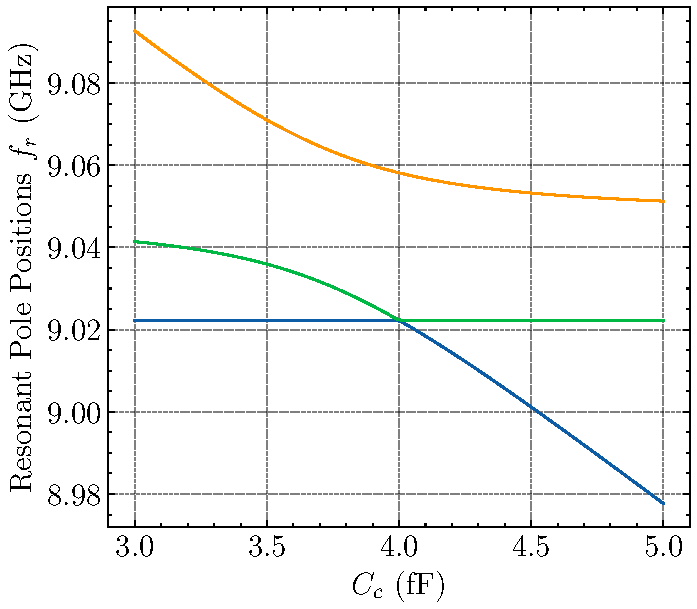
\includegraphics[width=0.5\textwidth]{figures/tetra_poles.pdf}
    \caption{Resonance frequencies of the network in Fig.\ \ref{fig:tetrahedral_circuit} for the parameters $C=$ 70 fF, $C_c=$ 4 fF, and $L_R=$ 4 nH while varying a single one of the coupling capacitors $C_c$. We can see that if a single coupling capacitance is not at 4 fF, the degeneracy is broken.}
    \label{fig:tetra_poles}
\end{figure}

\newpage
\section{Cascade Synthesis of the Ideal Transmission Line}\label{appendix:cascade_ideal_TL}
Here we consider the ideal lossless transmission line with two capacitors on either end as shown in Fig.\ \ref{fig:ideal_TL}. The result ends up being similar to the example in \cite[Appendix G]{Parra-Rodriguez_2018}, except here we have included the capacitors so that we have a positive definite DC residue.

\begin{figure}[h!]
    \centering
    \begin{circuitikz}[line width=1pt]
    \ctikzset{american}
    \ctikzset{bipoles/thickness=1, bipoles/length=1cm}
    \ctikzset{bipoles/crossing/size=0.5}
    \ctikzset { label/align = straight }

    \draw (0,1) to[short, o-] (0.5,1) to[C=$C_1$] (2,1) to[short, -o] (2.5,1) to[short,-o] (6,1) -- (6.5,1) to[C=$C_2$] (8,1) to[short, -o] (8.5,1);
    \draw (0,-.5) to[short,o-] (0.5,-.5) to[short, -o] (2.5,-.5) to[short, -o] (6,-.5) to[short,-o] (8.5,-.5);
    \node at (4.25,0.25) {$Z_0,\; \beta=\omega\sqrt{LC}$};
    
    \node at (4.25,-0.75) {$\ell$};
    \draw [-stealth](4.5,-0.75) -- (6,-0.75);
    \draw [-stealth](4,-0.75) -- (2.5,-0.75);

\end{circuitikz}
\caption{}
\label{fig:ideal_TL}
\end{figure}

The ABCD matrix of the above two-port network is \cite[Chapter 4]{Pozar_2011}:
\begin{equation}
    \mqty(A & B \\ C & D) = \mqty( 1 & 1/j\omega C_1 \\ 0 & 1) \mqty( \cos \beta\ell & jZ_0 \sin \beta\ell \\ jY_0\sin\beta\ell & \cos\beta\ell ) \mqty( 1 & 1/j\omega C_2 \\ 0 & 1)
\end{equation}
Using the ABCD parameters, we can compute the matrix elements of the two-port impedance parameter:
\begin{align}
    Z_{11} &= \frac{A}{C} = \frac{1}{j\omega C_1} - jZ_0 \cot\beta\ell \\
    Z_{12} &= Z_{21} = \frac{1}{C} = -jZ_0\csc\beta\ell \\ 
    Z_{22} &= \frac{D}{C} = \frac{1}{j\omega C_2} - jZ_0\cot\beta\ell
\end{align}
To find the cascade representation of this impedance function, we need to bring the above into partial fraction form. For this we can use the following series expansions \cite[1.421.3 and 1.422.3]{int_series_table}: 
\begin{align}
    \cot z &= \frac{1}{z} + 2z\sum_{k=1}^{\infty} \frac{1}{z^2 - \pi^2k^2} \\
    \csc z &= \frac{1}{z} + 2z\sum_{k=1}^{\infty} \frac{(-1)^{k}}{z^2 - \pi^2 k^2}
\end{align}
Putting together these expansions with the matrix elements of the impedance function for this two-port network, we find:
\begin{equation}
    \vb{Z}(s) = \frac{\vb{R}_0}{s} + \sum_{k=1}^{\infty} \frac{\vb{R}_k}{s^2 + \omega_k^2}
\end{equation}
where we have defined
\begin{align}
    \omega_k &= \frac{\pi^2 k^2}{L C \ell^2} \label{eq:ideal_TL_poles}\\
    \frac{1}{C_T} &= \frac{Z_0}{\ell\sqrt{L C}} \\
    \vb{R}_0 &= \mqty(C_1^{-1} + C_T^{-1} & C_T^{-1} \\ C_T^{-1} & C_2^{-1} + C_T^{-1}) \\
    \vb{R}_k &= \frac{2}{C_T} \mqty(1 & (-1)^k \\ (-1)^k & 1) = \frac{2}{C_T} \mqty(1 \\ (-1)^k) \Big(1 \quad (-1)^k\Big)
\end{align}

Now we can attempt to construct the CL cascade that corresponds to this circuit as described in Section \ref{section:cascade_synthesis}. The turns ratio matrix $\vb{R}$ for this network has the form:
\begin{equation}
    \vb{R} = \sqrt{\frac{2}{C_T}} \mqty(1 & -1 \\ 1 & 1 \\ \vdots & \vdots)
\end{equation}
where the two rows shown in the matrix are repeated infinitely. The port-resonance block of the capacitance matrix is given by (\ref{eq:impedance_cap}):
\begin{equation}
    -\vb{R}_0^{-1}\vb{R}^T = \frac{1}{C_{\Sigma}}\sqrt{\frac{2}{C_T}} \mqty( -C_1 C_T & -2C_1C_2 - C_1C_T & \dots \\ -C_2C_T & 2C_1C_2 + C_2C_T & \dots )
\end{equation}
where now the two columns are repeated infinitely. If we take this Maxwell capacitance and convert it to the mutual capacitance matrix, the capacitances in the mutual matrix correspond to the capacitive elements in the cascade representation of this network. For this case, as we take into account more poles, the capacitances shunting the ports of the cascade network will diverge. We can see this for two different parameter regimes in Fig.\ \ref{fig:ideal_TL_shunt_cap}.

\begin{figure}[h!]
    \centering
    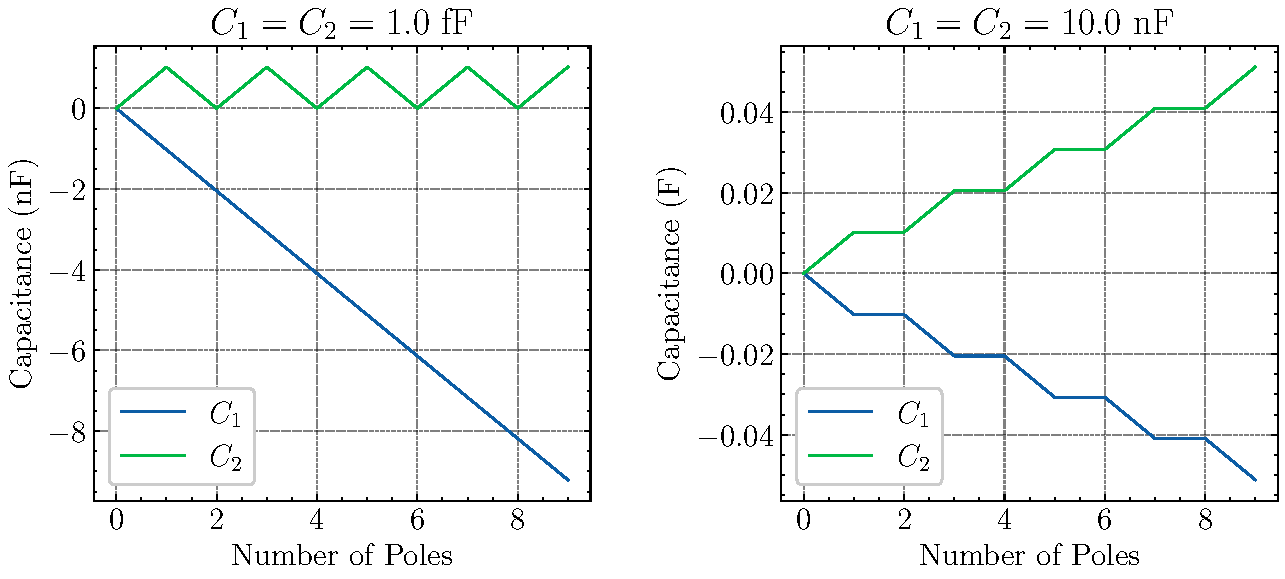
\includegraphics[width=\textwidth]{figures/ideal_TL_shunt_cap.pdf}
    \caption{Cascade representation shunt capacitance divergence for a transmission line with $L = $ 0.438 $\mu$H/m, $C = $ 0.159 nF/m, and $\ell =$ 12 mm. On the left, we have the case of $C_1 \ll C_T$ and on the right, we have $C_1 \gg C_T$.}
    \label{fig:ideal_TL_shunt_cap}
\end{figure}

In general, these divergences in the elements of the cascade representation are not encountered since we will always work with a finite number of poles. As long as we choose the poles that are within the relevant frequency range of our device, this should not cause any problems. 

\newpage
\section{Capacitance Matrix Comparison Between Q3D and HFSS}\label{appendix:q3d_vs_hfss}

Tables containing the capacitance matrix comparisons between the Q3D and HFSS simulations of the model shown in Fig.\ \ref{fig:xmon_brick}.

\renewcommand{\arraystretch}{1.5}
\begin{table}[h!]
    \centering
    \begin{tabular}{|r|r|r|r|r|r|}
    \hline
    Island  & Xmon    & Control & CPW1    & CPW2    & CPW2    \\ \hline
    Xmon    & 107.677 & -0.161  & -4.591  & -4.599  & -4.591  \\ \hline
    Control & -0.161  & 205.059 & -0.172  & -0.020  & -0.024  \\ \hline
    CPW1    & -4.591  & -0.172  & 188.247 & -0.278  & -0.078  \\ \hline
    CPW2    & -4.599  & -0.020  & -0.278  & 188.096 & -0.274  \\ \hline
    CPW3    & -4.591  & -0.024  & -0.078  & -0.274  & 188.211 \\ \hline
    \end{tabular}
    \caption{Maxwell capacitance matrix in units of fF for the Q3D simulation.}
\end{table}

\begin{table}[h!]
    \centering
    \begin{tabular}{|r|r|r|r|r|r|}
    \hline
    Port    & Xmon    & Control & CPW1    & CPW2    & CPW2    \\ \hline
    Xmon    & 115.226 & -0.150  & -4.323  & -4.353  & -4.350  \\ \hline
    Control & -0.150  & 203.097 & -0.155  & -0.015  & -0.017  \\ \hline
    CPW1    & -4.323  & -0.155  & 181.583 & -0.233  & -0.061  \\ \hline
    CPW2    & -4.353  & -0.015  & -0.233  & 183.722 & -0.234  \\ \hline
    CPW3    & -4.350  & -0.017  & -0.061  & -0.234  & 184.450 \\ \hline
    \end{tabular}
    \caption{Maxwell capacitance matrix in units of fF extracted from the HFSS simulation using the fit of the impedance shown in Fig.\ \ref{fig:xmon_fit}.}
\end{table}

\begin{table}[h!]
    \centering
    \begin{tabular}{|r|r|r|r|r|r|}
    \hline
    Island/Port & Xmon   & Control & CPW1    & CPW2    & CPW2    \\ \hline
    Xmon        & 7.011 \% & -6.933 \%&     -5.857 \%  &  -5.356 \%  &  -5.246 \%  \\ \hline
    Control     & -6.933 \% & -0.957 \% &   -9.738 \%  & -24.805 \% &  -31.562 \% \\ \hline
    CPW1        & -5.857 \% & -9.738 \% &   -3.540 \%  & -16.344 \% &  -22.103 \% \\ \hline
    CPW2        & -5.356 \% & -24.805 \% & -16.344 \% &   -2.326 \%  & -14.519 \% \\ \hline
    CPW3        & -5.246 \% & -31.562 \% & -22.103 \% &  -14.519 \% &   -1.998 \%  \\ \hline
    \end{tabular}
    \caption{Percent increase/decrease in the Maxwell capacitance elements from HFSS compared to Q3D.}
\end{table}


\newpage
\section[Decay of Coupling Rates for Networks with Banded Capacitance Matrices]{Decay of Coupling Rates for Networks with\\ Banded Capacitance Matrices}\label{appendix:banded_cap}

Consider a rectangular $N \times M$ grid of nodes. Each node has it's own shunt capacitance to ground as well as capacitors connecting it to its nearest neighbors. Notably, the capacitance matrix for such a network is of size $NM \times NM$ and is banded with bandwidth of $k=\min\{N,M\}$. Banded matrices have the property that the matrix elements of the inverse decay exponentially to zero as you move further from the diagonal \cite{banded_1, banded_2}. Since the coupling rates between the nodes are dependent on the inverse of the capacitance matrix (\ref{eq:node_coupling}), we expect that as you move further from a node in this type of network, the coupling rates will decay exponentially. Two examples of this are shown in Fig.\ \ref{fig:2x10_grid_cap} and Fig.\ \ref{fig:10x10_grid_cap}. In reality, the presence of long range capacitive coupling will change this, and it should be taken into account when modeling grids of qubits.

\begin{figure}[h!]
    \centering
    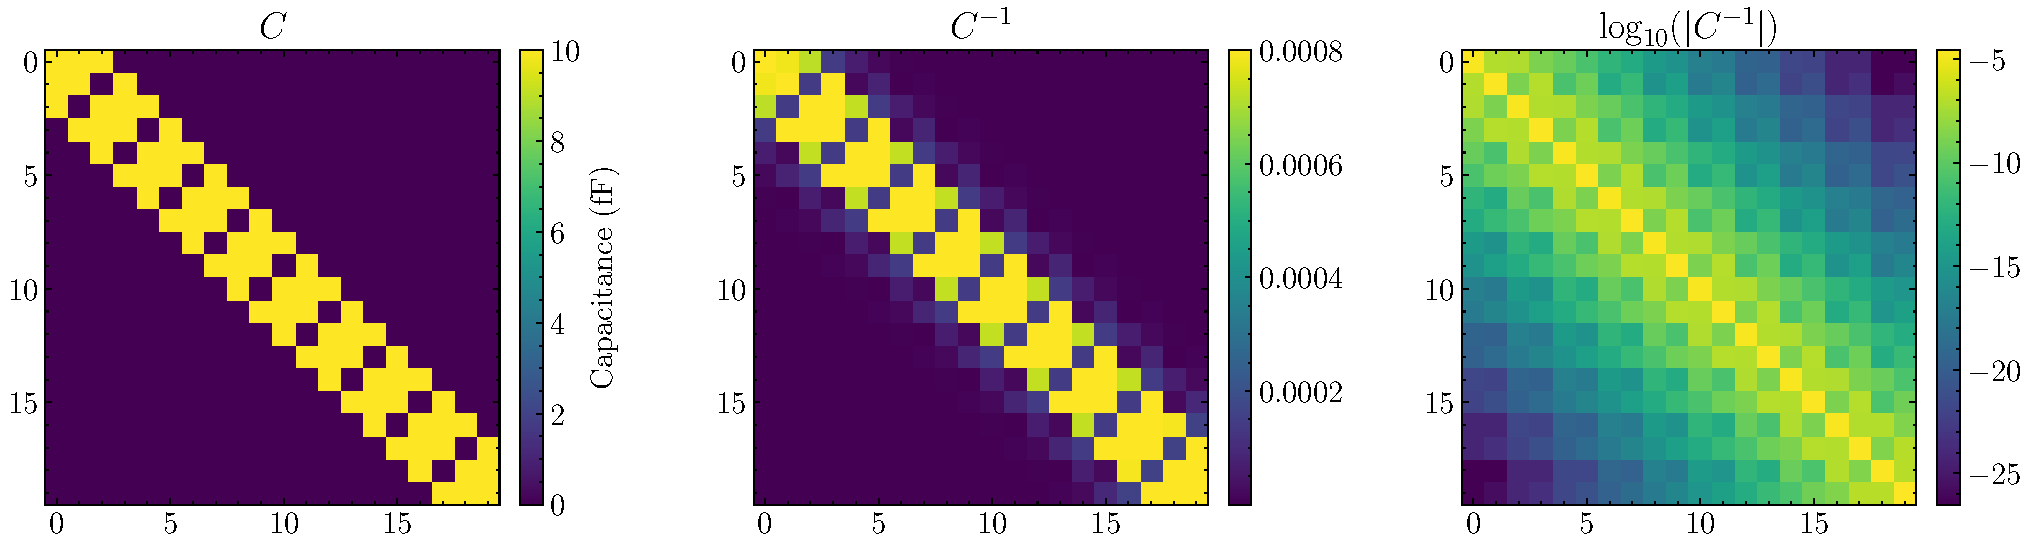
\includegraphics[width=\textwidth]{figures/2x10_grid_cap.pdf}
    \caption{Capacitance matrix and its inverse of a $2\times 10$ grid of nodes. The ground shunt capacitances of the nodes are $C_s=$ 100 fF, and the coupling capacitance to nearest neighbor nodes is $C_c =$ 10 fF.}
    \label{fig:2x10_grid_cap}
\end{figure}

\begin{figure}[h!]
    \centering
    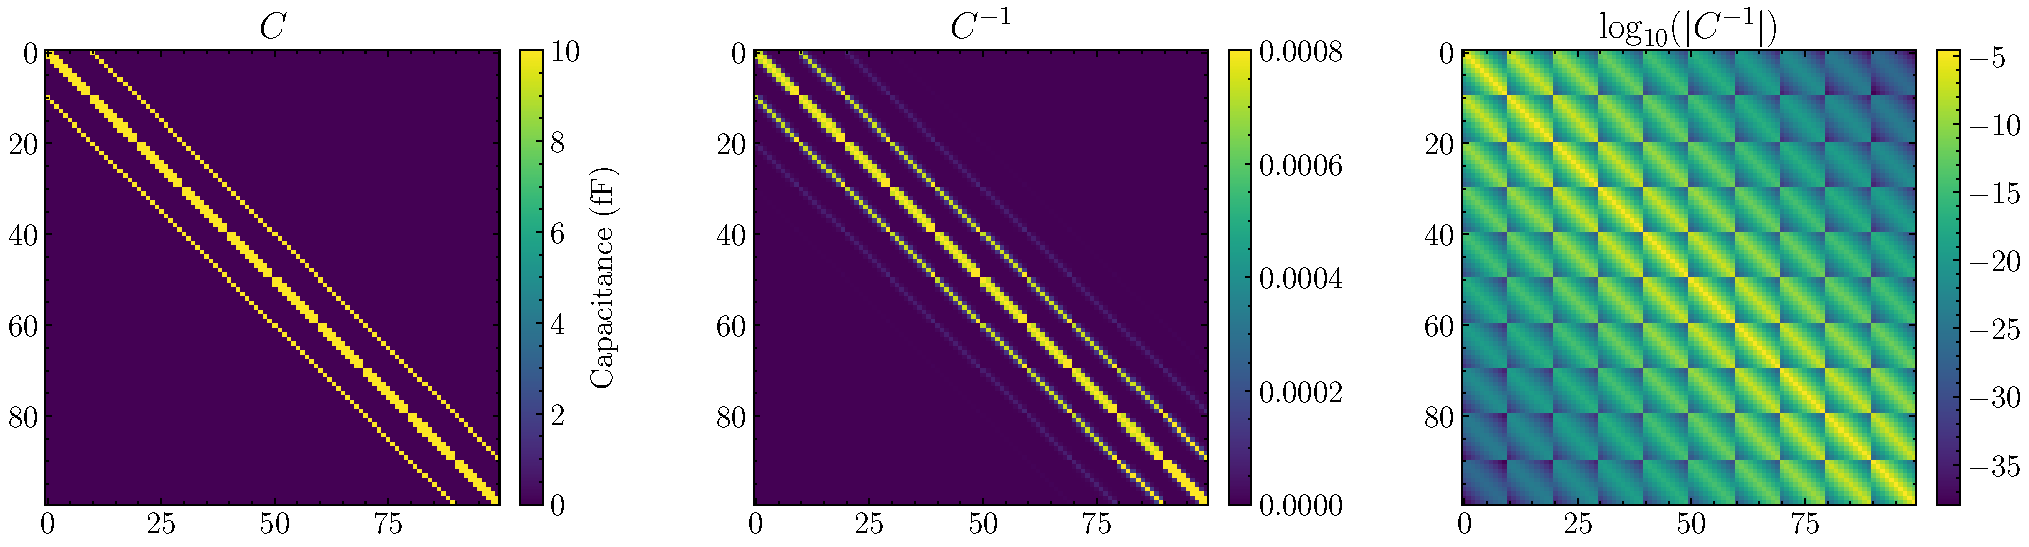
\includegraphics[width=\textwidth]{figures/10x10_grid_cap.pdf}
    \caption{Same as Fig.\ \ref{fig:2x10_grid_cap} but now for a $10 \times 10$ grid of nodes.}
    \label{fig:10x10_grid_cap}
\end{figure}